\documentclass[13pt]{beamer}
\usetheme[nat,greyfoot,footstyle=low,headstyle=institute,style=alternative]{Frederiksberg}

\usepackage[utf8]{inputenc}
\usepackage[english]{babel}
\usepackage{times}

\usepackage{amsmath}
\usepackage{amssymb}

\usepackage{xcolor}
\usepackage{color}
\usepackage{minted}
\setminted{frame=lines,linenos,framesep=2mm,fontsize=\small}

\usepackage{url}
\def\CC{{C\nolinebreak[4]\hspace{-.05em}\raisebox{.4ex}{\tiny ++}}}

\usepackage{pgfplots}
\usepgfplotslibrary{units}
\pgfplotsset{compat=newest}

\pgfplotsset{
  every axis plot post/.style={/pgf/number format/fixed}
}
\usepackage{graphicx}
\usepackage[caption=false,font=footnotesize]{subfig}
\newsubfloat{figure}



\normalfont
%\usepackage[T1]{fontenc}
\renewcommand{\ttdefault}{cmtt}
\usepackage{booktabs, caption, siunitx}

\usepackage{tikz}


\usepackage[labelsep=period]{caption}

\usetikzlibrary{calc}
\usetikzlibrary{fit}
\usetikzlibrary{positioning}
\usepgfplotslibrary{units}
\pgfplotsset{compat=newest}

\usetikzlibrary{decorations.markings}
\usetikzlibrary{arrows}
\usetikzlibrary{shapes.geometric}

\usepackage{ifthen}
\pgfkeys{
  /sevenseg/.is family, /sevenseg,
  slant/.estore in      = \sevensegSlant,     % vertical slant in degrees
  size/.estore in       = \sevensegSize,      % length of a segment
  shrink/.estore in     = \sevensegShrink,    % avoids overlapping of segments
  line width/.estore in = \sevensegLinewidth, % thickness of the segments
  line cap/.estore in   = \sevensegLinecap,   % end cap style rect, round, butt
  oncolor/.estore in    = \sevensegOncolor,   % color of an ON segment
  offcolor/.estore in   = \sevensegOffcolor,  % color of an OFF segment
}

\pgfkeys{
  /sevenseg,
  default/.style={
    slant = 0,
    size = 1em,
    shrink = 0.2,
    line width = 0.3em,
    line cap = butt,
    oncolor = green!50!black,
    offcolor = white!75!black
  }
}
\newcommand{\sevenseg}[2][]% options values
{%
\pgfkeys{/sevenseg, default, #1}%
\def\sevensegarray{#2}%
  \begin{tikzpicture}%
    % first define the position of the 6 corner points
    \path (0,0) ++(0,0)                             coordinate (P1);
    \path (0,0) ++(\sevensegSize,0)                 coordinate (P2);
    \path (0,0) ++(90-\sevensegSlant:\sevensegSize) coordinate (P3);
    \path (P2)  ++(90-\sevensegSlant:\sevensegSize) coordinate (P4);
    \path (P3)  ++(90-\sevensegSlant:\sevensegSize) coordinate (P5);
    \path (P4)  ++(90-\sevensegSlant:\sevensegSize) coordinate (P6);
    % then step through the 1/0 values in the segment array
    \foreach \i in {0,...,6}%
    {
      \pgfmathparse{\sevensegarray[\i]}
      \ifthenelse{\equal{\pgfmathresult}{1}}%
        {\let\mycolor=\sevensegOncolor}%  segment is on
        {\let\mycolor=\sevensegOffcolor}% segment is off
      \tikzstyle{segstyle} = [draw=\mycolor, line width = \sevensegLinewidth,
                              line cap = \sevensegLinecap]
      %-----------------------
      \ifthenelse{\equal{\i}{0}}{\path[segstyle]
        (${1-\sevensegShrink}*(P5)+\sevensegShrink*(P6)$)
        -- ($\sevensegShrink*(P5)+{1-\sevensegShrink}*(P6)$);}{} % a
      \ifthenelse{\equal{\i}{1}}{\path[segstyle]
        (${1-\sevensegShrink}*(P6)+\sevensegShrink*(P4)$)
        -- ($\sevensegShrink*(P6)+{1-\sevensegShrink}*(P4)$);}{} % b
      \ifthenelse{\equal{\i}{2}}{\path[segstyle]
        (${1-\sevensegShrink}*(P4)+\sevensegShrink*(P2)$)
        -- ($\sevensegShrink*(P4)+{1-\sevensegShrink}*(P2)$);}{} % c
      \ifthenelse{\equal{\i}{3}}{\path[segstyle]
        (${1-\sevensegShrink}*(P1)+\sevensegShrink*(P2)$)
        -- ($\sevensegShrink*(P1)+{1-\sevensegShrink}*(P2)$);}{} % d
      \ifthenelse{\equal{\i}{4}}{\path[segstyle]
        (${1-\sevensegShrink}*(P1)+\sevensegShrink*(P3)$)
        -- ($\sevensegShrink*(P1)+{1-\sevensegShrink}*(P3)$);}{} % e
      \ifthenelse{\equal{\i}{5}}{\path[segstyle]
        (${1-\sevensegShrink}*(P3)+\sevensegShrink*(P5)$)
        -- ($\sevensegShrink*(P3)+{1-\sevensegShrink}*(P5)$);}{} % f
      \ifthenelse{\equal{\i}{6}}{\path[segstyle]
        (${1-\sevensegShrink}*(P3)+\sevensegShrink*(P4)$)
        -- ($\sevensegShrink*(P3)+{1-\sevensegShrink}*(P4)$);}{} % g
    }
  \end{tikzpicture}%
}

% \newcommand{\sevensegnum}[2][]% sample characvters
% {%
%   \ifthenelse{\equal{#2}{0}}{\sevenseg[#1]{{1,1,1,1,1,1,0,}}}{%
%   \ifthenelse{\equal{#2}{1}}{\sevenseg[#1]{{0,1,1,0,0,0,0,}}}{%
%   \ifthenelse{\equal{#2}{2}}{\sevenseg[#1]{{1,1,0,1,1,0,1,}}}{%
%   \ifthenelse{\equal{#2}{3}}{\sevenseg[#1]{{1,1,1,1,0,0,1,}}}{%
%   \ifthenelse{\equal{#2}{4}}{\sevenseg[#1]{{0,1,1,0,0,1,1,}}}{%
%   \ifthenelse{\equal{#2}{5}}{\sevenseg[#1]{{1,0,1,1,0,1,1,}}}{%
%   \ifthenelse{\equal{#2}{6}}{\sevenseg[#1]{{1,0,1,1,1,1,1,}}}{%
%   \ifthenelse{\equal{#2}{7}}{\sevenseg[#1]{{1,1,1,0,0,0,0,}}}{%
%   \ifthenelse{\equal{#2}{8}}{\sevenseg[#1]{{1,1,1,1,1,1,1,}}}{%
%   \ifthenelse{\equal{#2}{9}}{\sevenseg[#1]{{1,1,1,1,0,1,1,}}}{%
%   \ifthenelse{\equal{#2}{A}}{\sevenseg[#1]{{1,1,1,0,1,1,1,}}}{%
%   \ifthenelse{\equal{#2}{B}}{\sevenseg[#1]{{0,0,1,1,1,1,1,}}}{%
%   \ifthenelse{\equal{#2}{C}}{\sevenseg[#1]{{0,0,0,1,1,0,1,}}}{%
%   \ifthenelse{\equal{#2}{D}}{\sevenseg[#1]{{0,1,1,1,1,0,1,}}}{%
%   \ifthenelse{\equal{#2}{E}}{\sevenseg[#1]{{1,0,0,1,1,1,1,}}}{%
%   \ifthenelse{\equal{#2}{F}}{\sevenseg[#1]{{1,0,0,0,1,1,1,}}}{%
%   {\sevenseg[#1]{{0,0,0,0,0,0,0,}}}}}}}}}}}}}}}}}}}%
% }

\tikzset{
  myarrow/.style={
    draw=black,
    thick,
    ->,
    shorten <=3pt,
    shorten >=3pt,
  },
  mycircle/.style={
    draw=black,
    shape=circle,
    very thick,
    inner sep=3pt,
    inner ysep=5pt,
    text width=0.75cm,
    align=center,
    minimum size=0.75cm,
    rounded corners,
  },
  mytriangle/.style={
    draw=black,
    regular polygon,
    regular polygon sides=3,
    align=center,
    rounded corners,
    very thick,
    inner sep=3pt,
  },
  myrectangle/.style={
    draw=black,
    shape=rectangle,
    very thick,
    rounded corners,
    align=center,
    inner sep=7pt,
    inner ysep=7pt,
    text width=2.1cm,
    minimum size=0.5cm,
    minimum height=1.5cm,
    font=\footnotesize
  },
  mysquare/.style={
    draw=black,
    shape=rectangle,
    very thick,
    rounded corners,
    align=center,
    inner sep=7pt,
    inner ysep=7pt,
    font=\footnotesize
  }
}

\pgfplotsset{
  every axis plot post/.style={/pgf/number format/fixed}
}












\title[Towards Automatic Program Specification Using SME Models]{Towards Automatic Program Specification \\ Using SME Models}
\subtitle{\tiny Communicating Process Architectures 2018 -- Technische Universität Dresden}
\author[A. Thegler]{Alberte Thegler}
\institute[Niels Bohr Institute]{Niels Bohr Institute, University of Copenhagen, Denmark}
\date[August 21]{21 August 2018}

\newcommand{\cspm}{CSP$_M$}

\begin{document}

\frame[plain]{\titlepage}

%%%%%%%
%%% TOC
% \begin{frame}{Table of Contents}
%   \begin{enumerate}
%     \item Why should we verify hardware?
%     \item What can SME do?
%     \item SMEIL
%     \item Simple example
%     \item CSPm process structure
%     \item Monitor process
%     \item Example continued
%     \item Results - time to verify in FDR4?
%     \item Conclusion
%     \item Future work
%   \end{enumerate}
% \end{frame}
%%% /TOC
%%%%%%%%

%%%%%%%%%%%%%%%%%%%%%%
%%% Why should we verify hardware?
\begin{frame}{Why should we verify hardware?}
  \begin{block}{Ariane-5}
    4th June 1996
  \end{block}

  \pause

  \begin{block}{}
     Total failure on launch
  \end{block}

  \pause

  \begin{block}{}
     Converting a 64-bit floating point number to signed 16-bit integer.
  \end{block}

  \pause

  \begin{block}{}
    Overflow caused the self-destruct mechanism in both primary and backup computer
  \end{block}

  \pause

  \begin{block}{}
     No people where harmed
  \end{block}

\end{frame}

\begin{frame}{Why should we verify hardware?}
  \begin{block}{The Patriot Missile Failure}
    25th February 1991 in the Persian Gulf war
  \end{block}

  \pause

  \begin{block}{}
     A Patriot missile failed to intercept an incomming "Scud" which struck a U.S Army barracks, killing 28 soldiers.
  \end{block}

  \pause

  \begin{block}{}
     A bug in the system's weapons control computer caused an inaccurate tracking calculation.
     Conversion of time since last boot from an integer to a real number was performed using a 24 bit register.
  \end{block}

  \pause

  \begin{block}{}
     Inaccurate results == missile misses target
  \end{block}

\end{frame}
%%%
%%%%%%%%%%%%%%%%%%%%%%%
%
%%%%%%%%%%%%%%%%%%%%%%%%%%%%%%%%%%
%%% What can SME do?
\begin{frame}{What can SME do?}
 \begin{block}{}
   The SME model builds on the CSP algebra
 \end{block}
\end{frame}
%%
%%%%%%%%%%%%%%%%%%%%%%%%%%%%%%%%%%%%
%
%%%%%%%%%%%%%%%%%%%%%%%%%%%
%% SMEIL
\begin{frame}{SMEIL}
 \begin{block}{}
   You have just been introduced to SMEIL in the previous presentation
 \end{block}

 \pause

 \begin{block}{}
   We transpile from SMEIL to \cspm{}\\
   And then verify it in FDR4
 \end{block}

 \pause

 \begin{block}{}
   \begin{figure}[!ht]
  \centering
  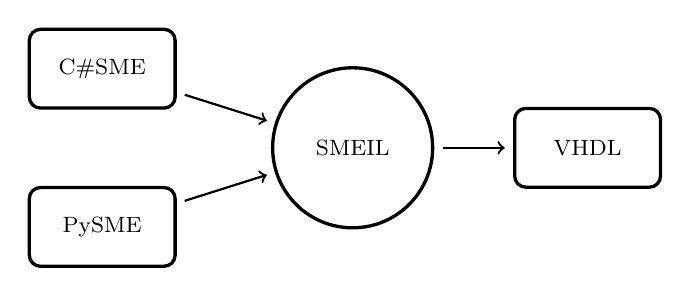
\begin{tikzpicture}[auto]
    \node[mycircle, minimum size=1.75cm, align=center, text width=1.75cm, font=\footnotesize]    (smeil)                                       {SMEIL};
    \node[myrectangle, text width=1.5cm, minimum height=1.0cm, inner sep=5pt, inner ysep=5pt] (csme)  [above left=-0.25cm and 1.5cm of smeil] {C\#SME};
    \node[myrectangle, text width=1.5cm, minimum height=1.0cm, inner sep=5pt, inner ysep=5pt] (pysme) [below left=-0.25cm and 1.5cm of smeil] {PySME};
    \node[myrectangle, text width=1.5cm, minimum height=1.0cm, inner sep=5pt, inner ysep=5pt] (vhdl)  [right=1.0cm of smeil]                {VHDL};

    \draw[myarrow] (csme)  -- (smeil);
    \draw[myarrow] (pysme) -- (smeil);
    \draw[myarrow] (smeil) -- (vhdl);
  \end{tikzpicture}
  \caption{SMEIL transpiler structure.}
  \label{fig:smeil_transpiler}
\end{figure}
 \end{block}
\end{frame}
%%
%%%%%%%%%%%%%%%%%%%%%%%%%%%%%%%%%%%%
%
%%%%%%%%%%%%%%%%%%%%%%%%%%%
%% Simple example
\begin{frame}{Simple example}
 \begin{block}{Seven Segment Display}
   Figure (Truls or something else?)
 \end{block}

\end{frame}

\begin{frame}{Seven Segment Display example}
 \begin{block}{}
   Write the seven segment circuit in SMEIL
 \end{block}

 \pause

 \begin{block}{}
  Transpile it to \cspm{}
 \end{block}

 \pause

 \begin{block}{}
  Verify in FDR4
 \end{block}

\end{frame}

\begin{frame}{Simple example}
 \begin{block}{What are we verifying}
   One seven segment example can only display the numbers 0-9. \\
   4 bits can represent the data, but also more than needed.
 \end{block}

 \pause

 \begin{block}{}
   We can verify that the values communicated to the seven segment displays does not exceed the expected values.
 \end{block}


\end{frame}


\begin{frame}{Simple example}
 \begin{block}{Seven Segments SMEIL Structure}
  SMEIL code
 \end{block}
\end{frame}

\begin{frame}{Simple example}
 \begin{block}{Seven Segments SMEIL Structure}
  \begin{figure}[!ht]
  \centering
  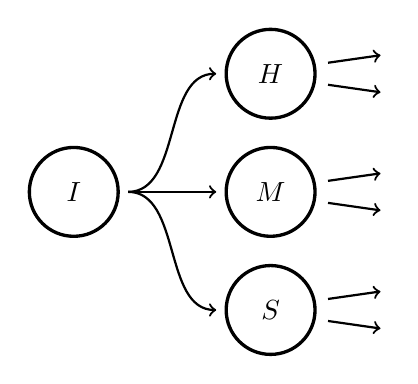
\begin{tikzpicture}
    \node [mycircle] (I) at (0,0) {$I$};

    \node [mycircle] (H) at (2.5,  1.50) {$H$};
    \node [mycircle] (M) at (2.5,  0.00) {$M$};
    \node [mycircle] (S) at (2.5, -1.50) {$S$};

    \draw [myarrow] (I) -- (M);

    \draw [myarrow, smooth] (I) to[out=0, in=180] (H);
    \draw [myarrow, smooth] (I) to[out=0, in=180] (S);

    % Output arrows without processes
    \draw [myarrow] (3.125,  1.625) -- (4.000,  1.750);
    \draw [myarrow] (3.125,  1.375) -- (4.000,  1.250);
    \draw [myarrow] (3.125,  0.125) -- (4.000,  0.250);
    \draw [myarrow] (3.125, -0.125) -- (4.000, -0.250);
    \draw [myarrow] (3.125, -1.375) -- (4.000, -1.250);
    \draw [myarrow] (3.125, -1.625) -- (4.000, -1.750);
  \end{tikzpicture}
  \caption{SMEIL network for a seven segment display clock. Each SMEIL process is represented by a cicle with a letter corresponding to the processes Input, Hours, Minutes and Seconds respectively.}
  \label{fig:smeil_network}
\end{figure}
 \end{block}
\end{frame}

%%
%%%%%%%%%%%%%%%%%%%%%%%%%%%%
%
%%%%%%%%%%%%%%%%%%%%%%%%%%%%%%
%% CSPm process structure
\begin{frame}{CSPm process structure}
 \begin{block}{}
   Code example
 \end{block}

\end{frame}
%%
%%%%%%%%%%%%%%%%%%%%%%%%%%%%%%%
%
%%%%%%%%%%%%%%%%%%%%%%%%%%%%
%% Monitor process
\begin{frame}{Monitor process}
 \begin{block}{}
   Code example
 \end{block}

\end{frame}
%%
%%%%%%%%%%%%%%%%%%%%%%%%%%%%%
%
%%%%%%%%%%%%%%%%%%%%%%%
%% Example continued
\begin{frame}{Example continued}
 \begin{block}{Run}
   All of the following CPU examples have been run on a Intel(R) Core(TM) i7-3770 CPU @ 3.40GHz.
   \vspace{5mm}

   The GPGPU examples are run on GeForce GTX 680 (OpenCL C 1.1).
   \vspace{5mm}

   All examples were run 10 times and the average was measured.
 \end{block}
\end{frame}
%%
%%%%%%%%%%%%%%%%%%%%%%%%%%%%%
%
%%%%%%%%%%%%%%%%%%%%%%%
%% Results - time to verify in FDR4?
\begin{frame}{Results - time to verify in FDR4?}
 \begin{block}{}
   The seven segment example have been run on a ...
   \vspace{5mm}

   The example were run x times and the average was measured.
 \end{block}
\end{frame}
%%
%%%%%%%%%%%%%%%%%%%%%%%%
%
%%%%%%%%%%%%%
%% Conclusion
\begin{frame}{Conclusion}
 \begin{block}{Productivity and performance}
  ....
 \end{block}
\end{frame}
%% /Conclusion
%%%%%%%%%%%%%%
%
%%%%%%%%%%%%%%
%% Future work
\begin{frame}{Future work}
 \begin{block}{DSL}
     ....
 \end{block}
\end{frame}
%% /Future work
%%%%%%%%%%%%%%%
%
%%%%%%%%%%%%%%%
%%%% Questions?
\begin{frame}{Questions?}
	\begin{block}{Comments?}
		Feel free to ask anything.
	\end{block}
\end{frame}
%%%% /Questions?
%%%%%%%%%%%%%%%%

\end{document}
